\documentclass[a4paper]{article}
\usepackage[top=1cm,bottom=2cm,left=2cm,right=2cm]{geometry}
\usepackage{multicol,caption}
\usepackage{lipsum}
\usepackage{graphicx}
\usepackage[parfill]{parskip}
\usepackage{authblk}
\usepackage{titlesec}
\usepackage{wrapfig}
\usepackage[utf8]{inputenc}

\newenvironment{Figure}
	{\par\medskip\noindent\minipage{\linewidth}}
	{\endminipage\par\medskip}

\titlespacing*{\section}
{0pt}{1.0ex plus 1ex minus .2ex}{0.0ex plus .2ex}
\titlespacing*{\subsection}
{0pt}{1.0ex plus 1ex minus .2ex}{0.0ex plus .2ex}
\titlespacing*{\subsubsection}
{0pt}{0.5ex plus 1ex minus .2ex}{0.0ex plus .2ex}

\title{Workshop I: Clinical Imaging}
\author{Andreas Bachmann, Carolina Duran, Dario Lenherr, Till Obrist, Mario Windler
	\\
	ZHAW Zurich University of Applied Sciences\\
	School of Engineering
}
\date{06. - 07.04.2018}


\begin{document}
	\maketitle
	
	%Body
	\begin{multicols*}{2}
		\section{Introduction}
			A 44-year-old male skier had a high velocity skiing accident. He got delivered to the hospital suffering from
			severe pain in his left knee. A lot of swelling and edema was discovered around his knee. He also had a valgus
			instability. His soft tissue was intact, the nerves weren’t damaged, and the patient was in a generally healthy
			condition.
			
			With the help of medical imaging technologies and other means of clinical diagnostics a treatment-strategy
			shall be defined. Also, a fitting after treatment will be determined.
		
		\section{Methods}
			\subsection{Physical examination}
				As a first step, the patients knee is assessed through classical physical examination.
				The knee was visually analyzed and palpated.
				
			\subsection{X-Rays}
				The patients knee is X-rayed and in both anterior-posterior as well as medial-lateral directions are X-ray
				images taken. To find any abnormalities in these images, it is recommended to follow the outlines of the
				bone and check for irregularities. This process is done for each bone on both X-ray images.
								
			\subsection{CT-Scans}
				All suspicions of additional lesions must be eliminated. Therefore, an additional CT scan is made.
				The CT-scans are again taken in both anterior-posterior as well as medial-lateral directions. There will
				be about 50 images taken for each direction which can be looked at separately. It is also usual to create
				a 3D reconstruction out of the CT-scans.
				
		\section{Results}
			\subsection{X-Rays}
				On Figure \ref{fig:xray} there are two fractures visible. The first fracture is a splintering of a part
				of the tibial bone on the lateral proximal position. The second fracture is the lateral proximal part
				of the tibial bone that was pressed in distal direction into the bone.
			
				\begin{Figure}
					\centering
					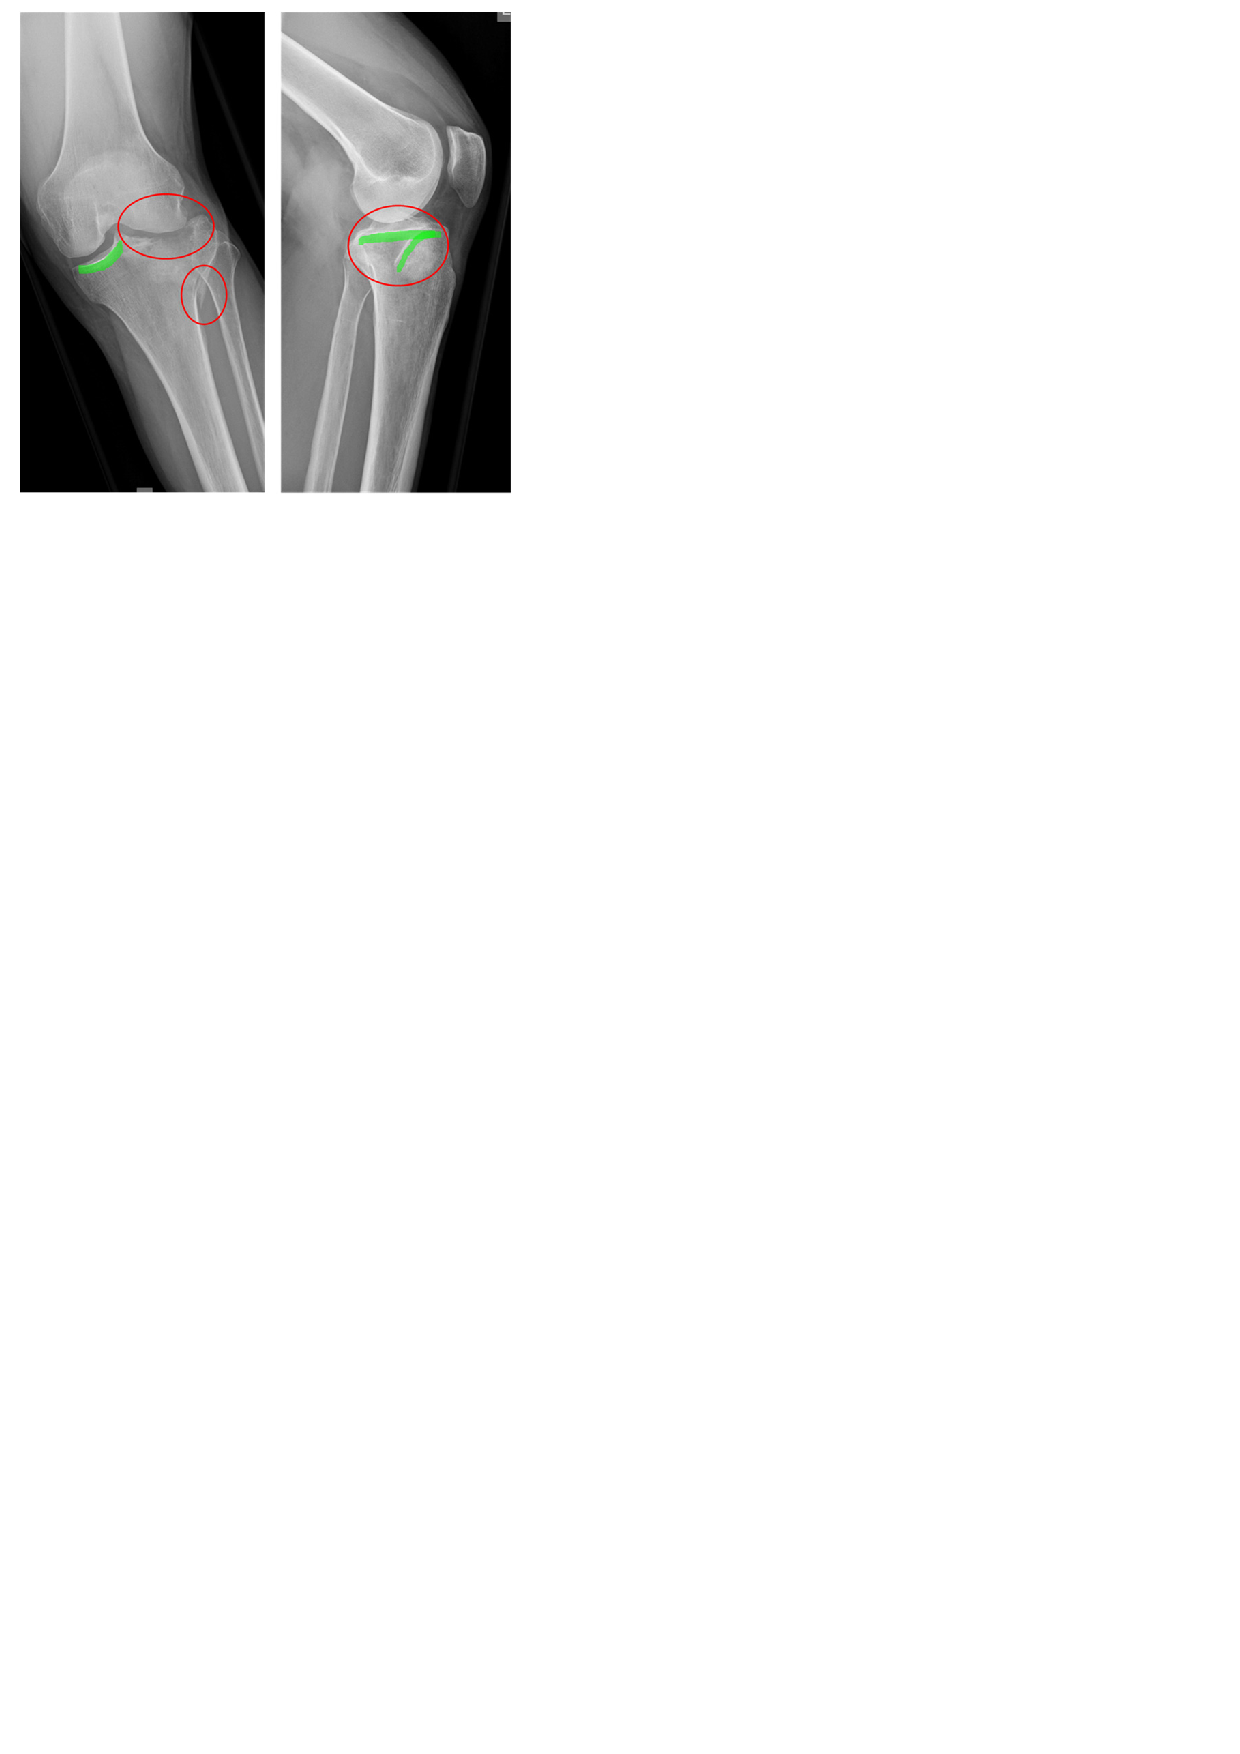
\includegraphics[trim={0.5cm 21.3cm 12.3cm 0},clip,width=7cm]{images/figure1_xray_knee.pdf}
					\captionof{figure}{X-ray of patient’s knee, AP an ML view.}
					\label{fig:xray}
				\end{Figure}
			
			\subsection{CT-Scans}
				In Figure \ref{fig:ct} you can see the 2D reconstruction of some images of the CT scan from
				anterior-posterior as well as medial-lateral directions. In these images the injuries are seen
				very well. It is also visible that the lateral ligaments are fortunately still intact.
			
				\begin{Figure}
					\centering
					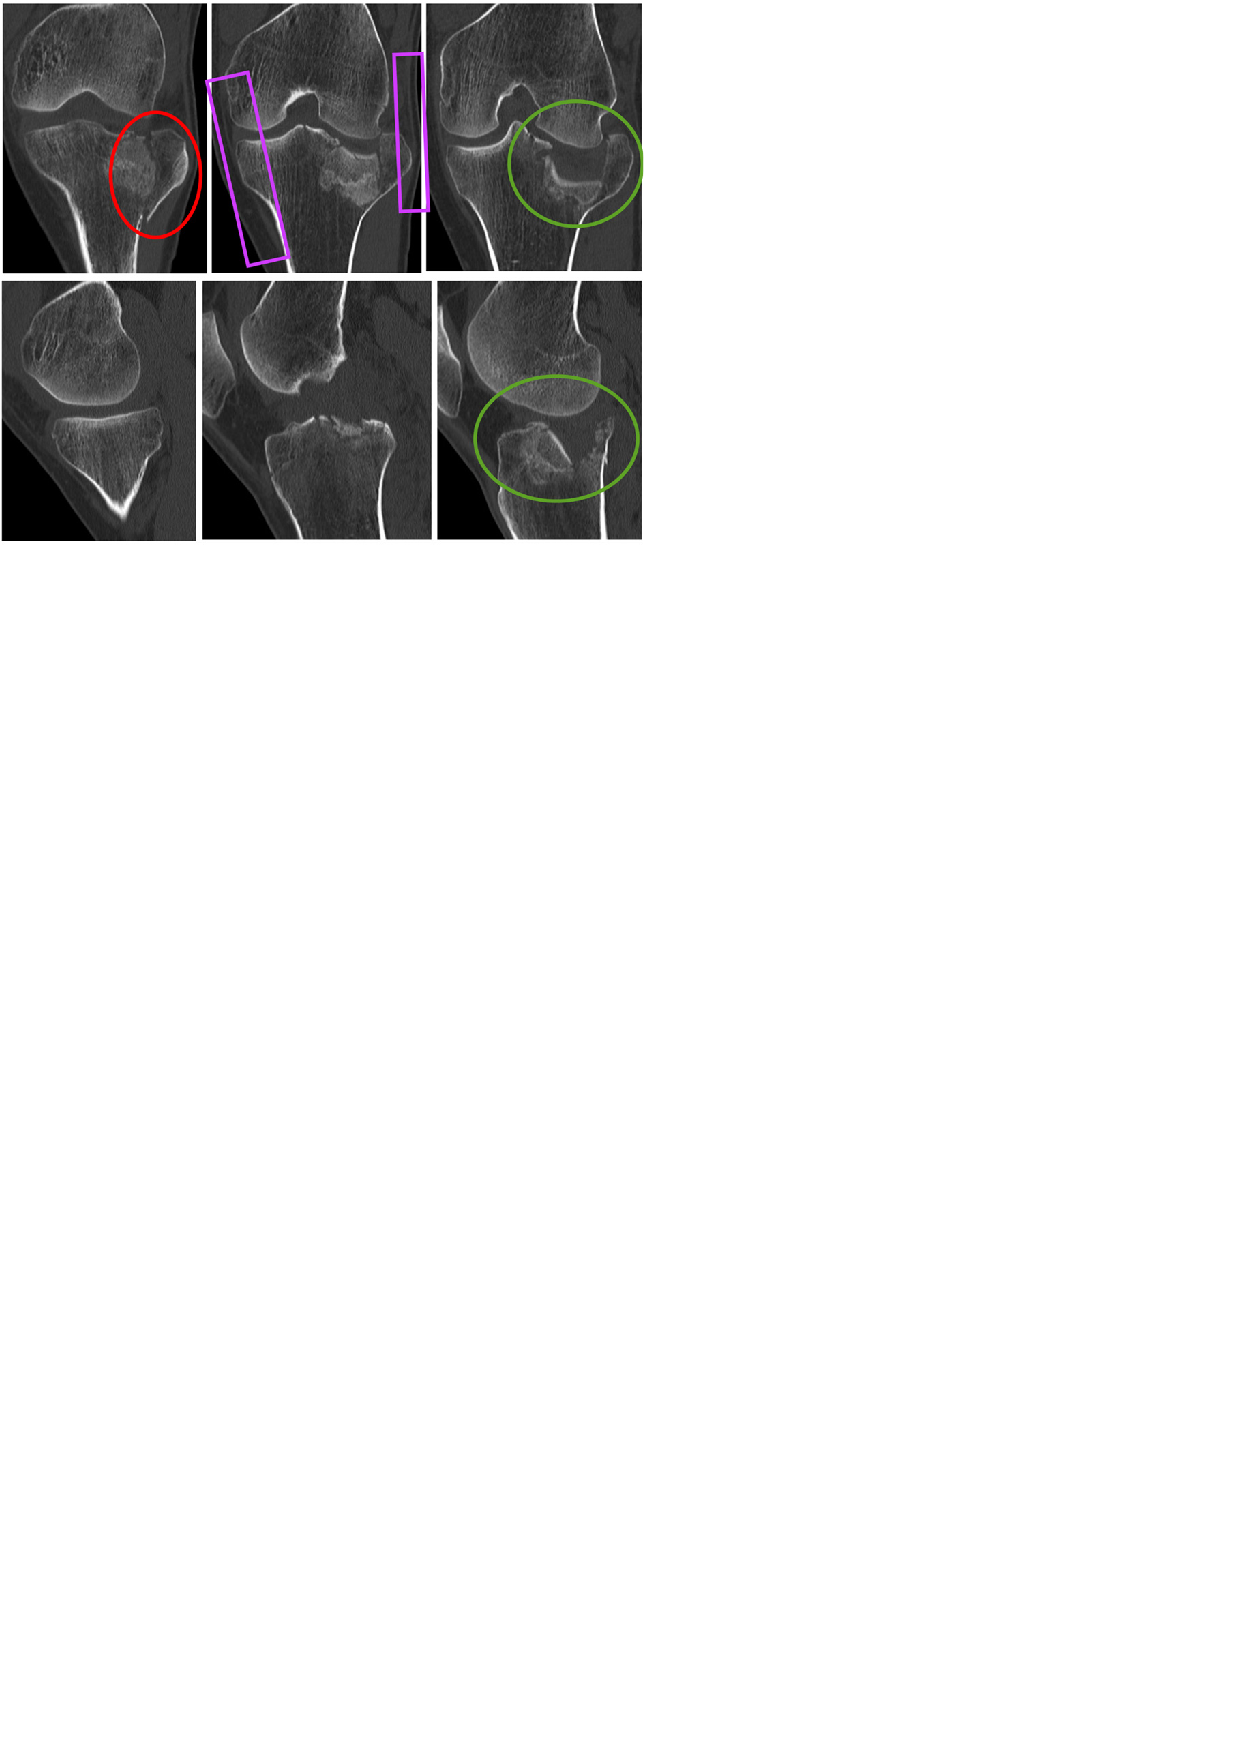
\includegraphics[trim={0cm 20.5cm 10cm 0},clip,width=7cm]{images/figure2_ct_scan.pdf}
					\captionof{figure}{2D reconstruction of some pictures from the CT scan.}
					\label{fig:ct}
				\end{Figure}
				
				The 3D reconstruction in Figure \ref{fig:3d} gives more details about the tibial fracture.
				Nevertheless, in the 2D reconstruction the ligaments and other soft tissue is better seen.
				
				\begin{Figure}
					\centering
					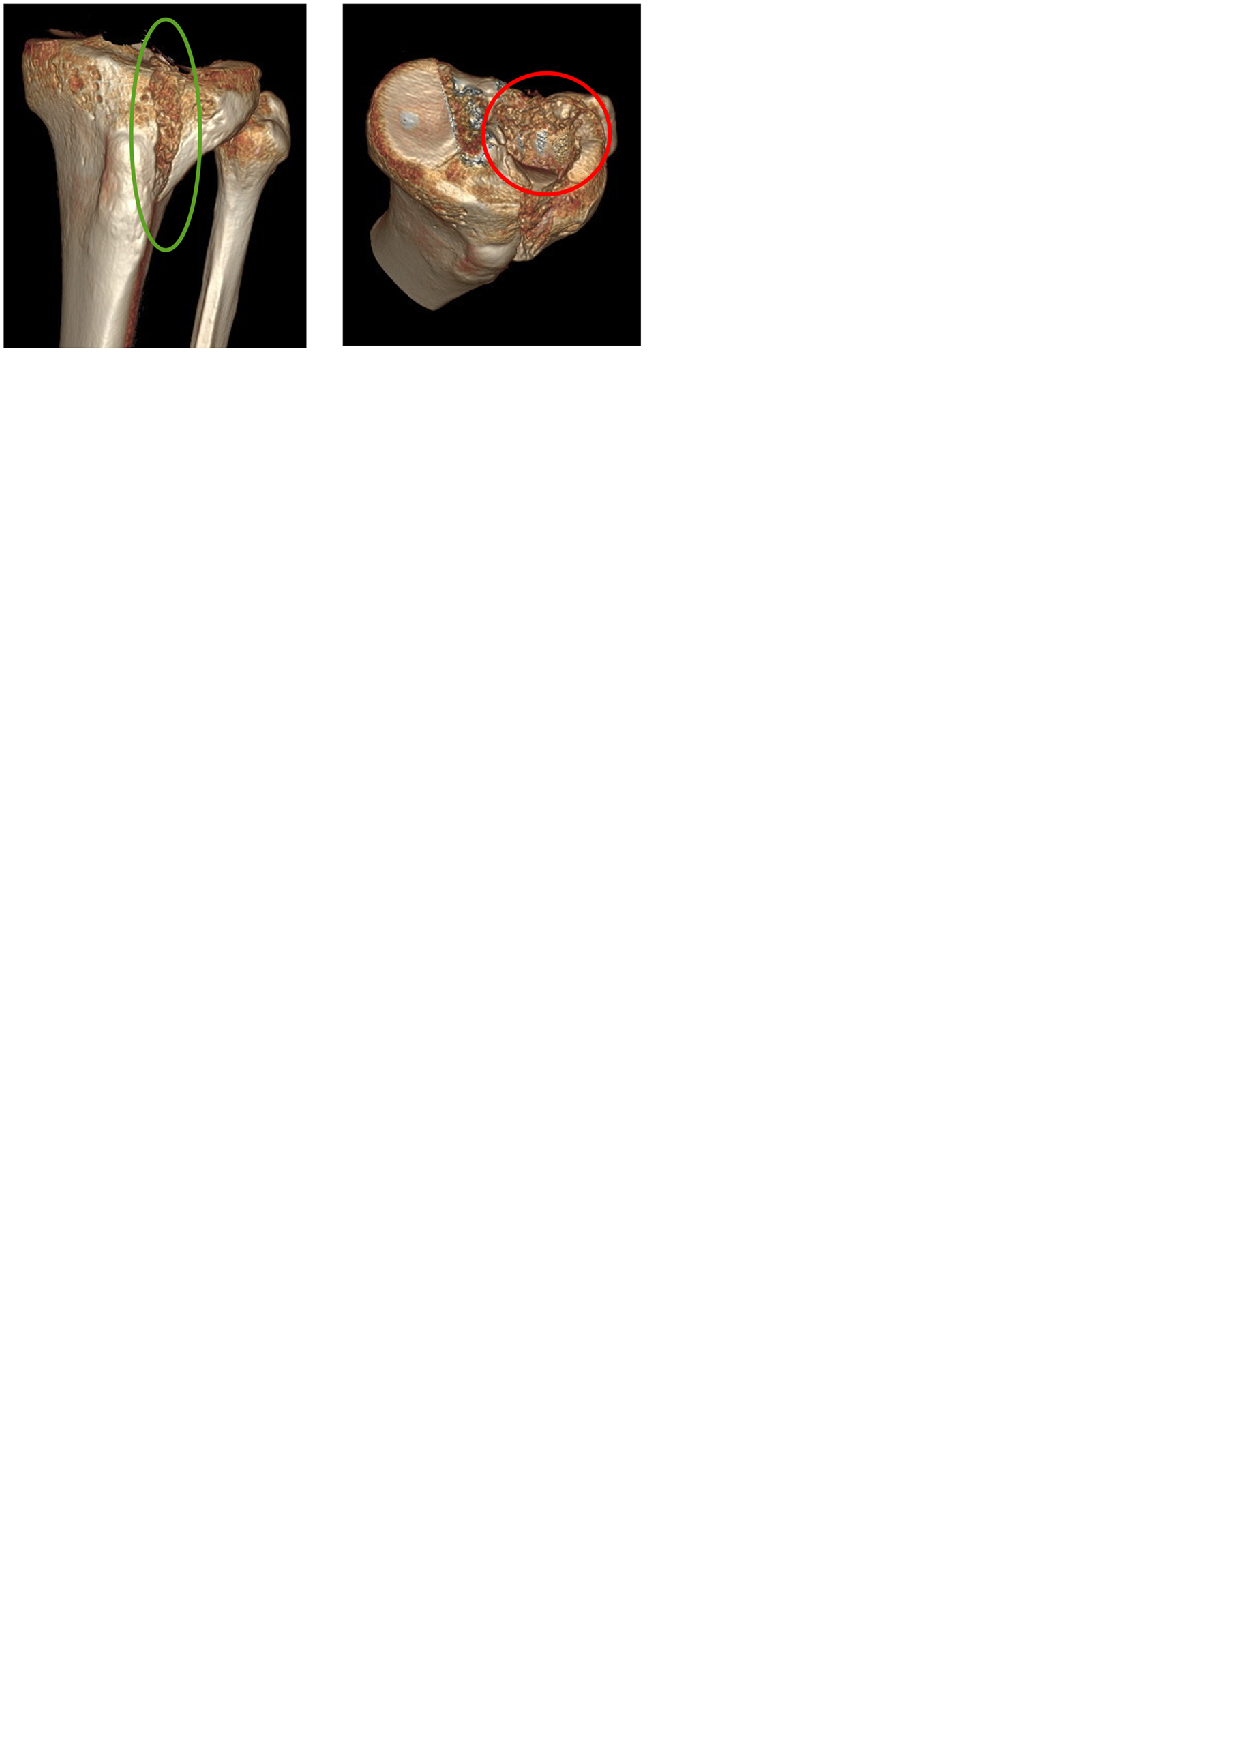
\includegraphics[trim={0cm 23.5cm 10cm 0},clip,width=7cm]{images/figure3_3d.pdf}
					\captionof{figure}{3D reconstruction of some pictures from the CT scan.}
					\label{fig:3d}
				\end{Figure}
				
		\section{Discussion}
			As the investigation has been completed some discussions have to be made. For example,
			the question about additional lesions must be discussed or the treatment strategy has
			to be established. These and more topics are discussed in chapter four.
			
			\subsection{Suspected additional lesions}
				As seen in the CT scans the ligaments are intact. Also, the meniscus is not injured.
				As the patient had a swelled knee but no suspicious colour of the knee, it can be said
				that there are no major injuries of the blood vessels.
				
			\subsection{Treatment strategy}
				According to the examination of the patient through the methods mentioned in chapter
				two, the suitable treatment strategy should be chosen.
			
				\subsubsection{Operative vs. conservative}
					Because the fracture is in a joint, a conservative treatment strategy isn’t beneficial
					for the patient. This is because trough the lack of motion during the treatment the joint
					will stiffen up. The rather large dislocation of the lateral condyle also suggests an
					operative treatment strategy. The operation bares many benefits in this case. The fracture
					can be reduced resulting in faster bone healing and the joint can be moved during the
					healing process assisting blood circulation.
					
				\subsubsection{Time of surgery}
					The patient has no other major problems. Therefore, the time of surgery can be chosen
					in a wider timeframe. This is beneficial for the patient because the operation can be
					planned in more detail and the swelling of the knee will be reduced by that time. 
					
				\subsubsection{Approach}
					The incision will be performed from the lateral side since it provides the best access
					to the damaged bone. Because the fracture is rather difficult to reduce a minimal invasive
					strategy will not work.
					
				\subsubsection{How to reduce and fix}
					The most lateral fractured part is removed to gain access to the dislocated condyle.
					The condyle is then pushed back in to place. The cavity created is filled with bone
					material to accelerate the bone formation process. 
					
				\subsubsection{Bone grafting\\(Autograft, Allograft, artificial)}
					To replace the missing bone, in this case the missing volume due to the compression,
					a surgical procedure named bone grafting needs to be performed. Different types of
					bone grafting may be autologous (bone from the patient’s own body), allograft (bone
					of a human cadaver) or artificial (made of hydroxyapatite or other naturally occurring
					and biocompatible substances) with similar mechanical properties to bone.
					
					To sustain stability and prevent the bone from collapsing, the condyle area needs to
					be supported. This is achieved with 5 screws, that redirects the load over the trauma
					plate.

			\subsection{After treatment}
				To ensure efficient healing of the bone, the load must be reduced to an absolute minimum
				at the beginning. During the healing process, the patient should be attending physical
				therapy. From time to time the patient can load the knee with an increased force. Within
				8 to 12 weeks, the bone has regenerated to a degree, where it can be loaded with 100\%
				of the body weight.
			
			\subsection{Expected longterm result}
				The bone healed completely without any complications as seen in Figure \ref{fig:xray-postop}.
				The trauma plate and the screws are held in place tightly and no damage is visible. The
				patient won’t have any issues with his left knee and will be able to make sportive activities.
				If not necessary, the trauma plate remains within the body. Performing an additional operation
				to remove the parts, the knee must be fully opened again, which might result in complications,
				for the knee is prone to infections.
				
				\begin{Figure}
					\centering
					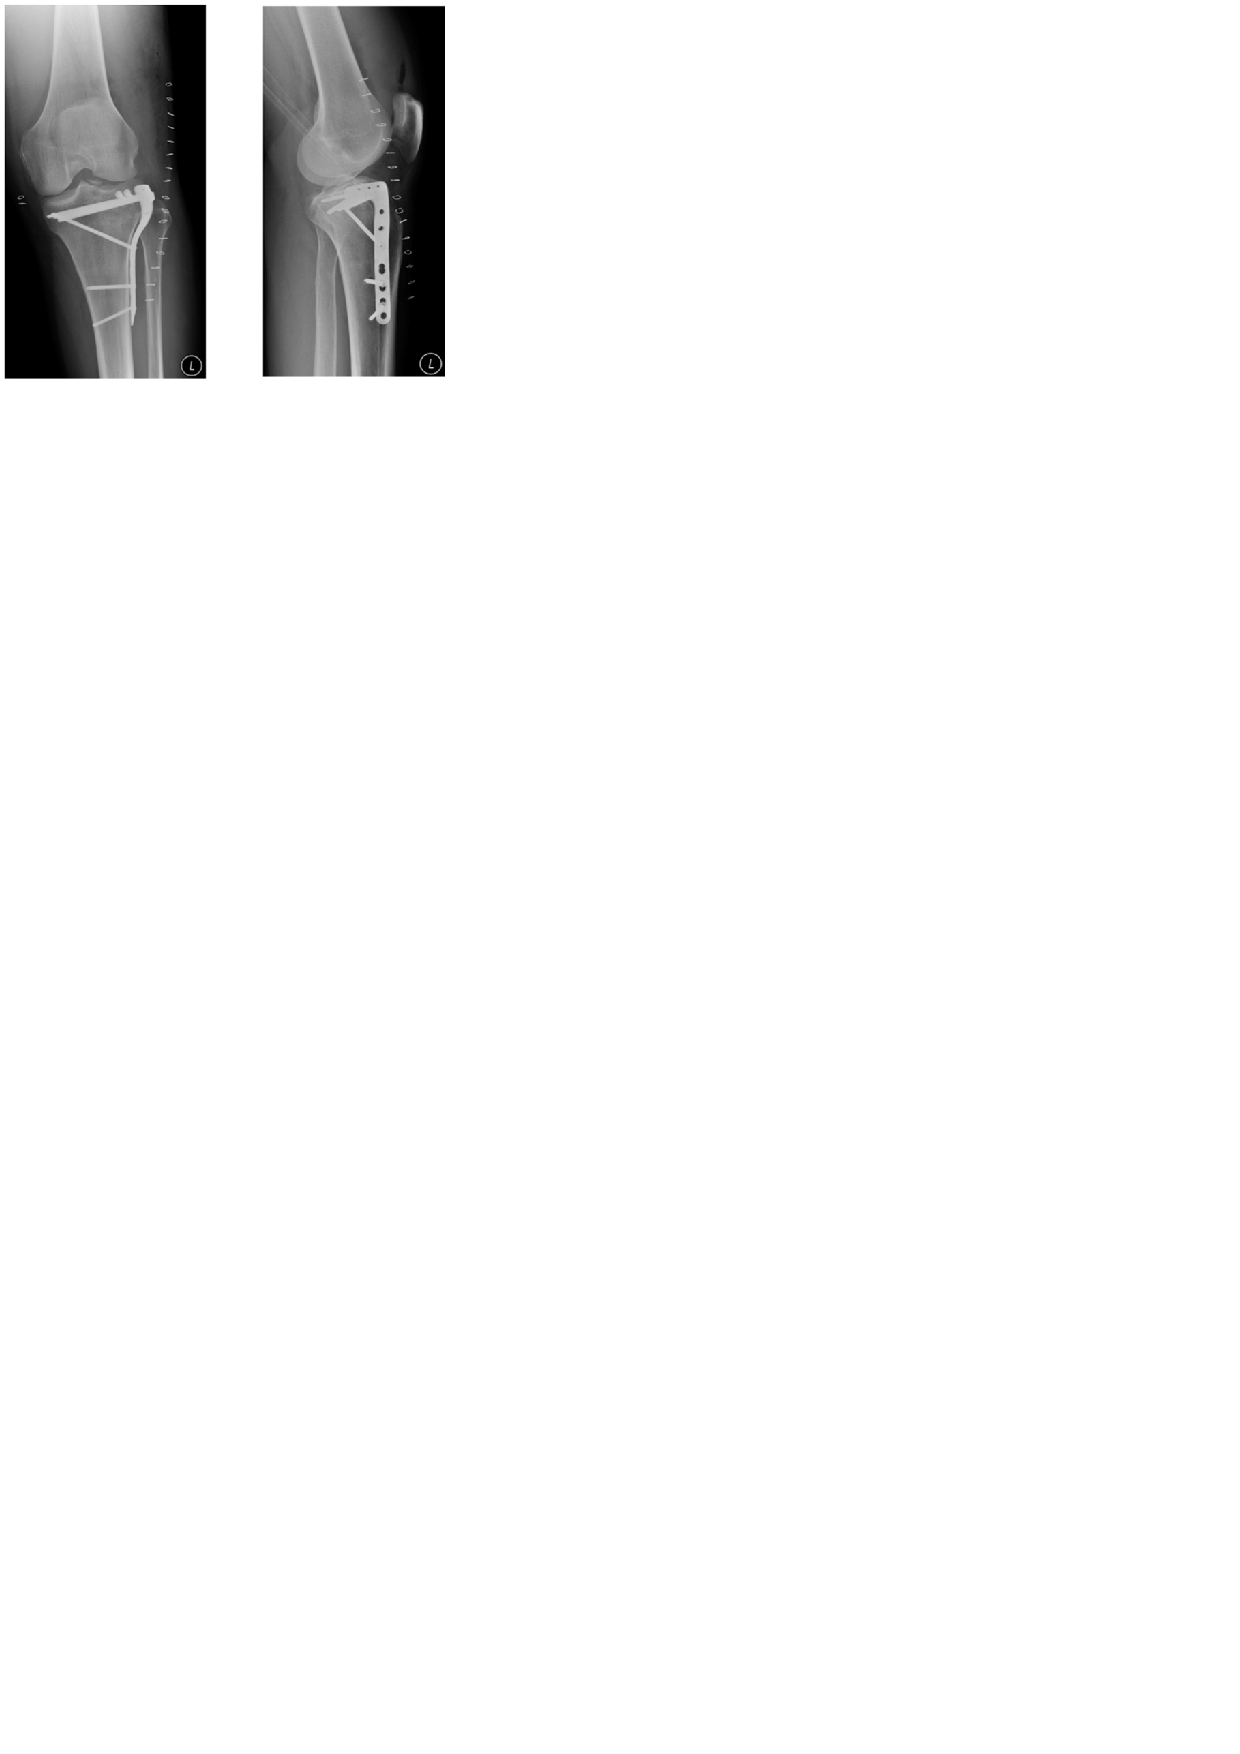
\includegraphics[trim={0cm 23.2cm 13.4cm 0},clip,width=7cm]{images/figure4_xray_postop.pdf}
					\captionof{figure}{Postoperative X-Rays of the left knee}
					\label{fig:xray-postop}
				\end{Figure}
			
	\end{multicols*}
\end{document}